\documentclass[t]{beamer}
\setbeamertemplate{navigation symbols}{} %no nav symbols
\usepackage{beamerthemeshadow}
\usepackage{pgf}
\usepackage{listing}
\usepackage{listings}
\usepackage{verbatim}
\usepackage{multirow}
\usetheme{Copenhagen} % Beamer theme v 3.0
\usecolortheme{whale} % Beamer color theme


\usepackage[boxed,linesnumbered,vlined,slide]{algorithm2eCustom}



\title[July Presentation 2011\hspace{14em}\insertframenumber/\inserttotalframenumber]{Rethinking Database Algorithms\\ for Phase Change Memory}
\author[Jeppe R. Thomsen]{Shimin Chen$^{1}$, Phillip B. Gibbons$^{1}$, Suman Nath$^{2}$}%\\ \small{jenslyn@cs.aau.dk}}
\institute{$^{1}$Intel Labs Pittsburgh, $^{2}$Microsoft Research}
\begin{document}
\begin{frame} % Cover slide
\titlepage
\end{frame}
% Instead, you can use \frame{\titlepage}} (Beamer v 2.2 macro)
%
%\section{Introduction} % Bookmark information
%
%\begin{frame}[red]
%\frametitle{Overview}
%\Large
%
%\end{frame}



\section{Introduction} % Bookmark information

\subsection{Overview} % Bookmark information, displayed in the progress tree

\begin{frame}[red] %hmm.. thought i could change colour here :S
\frametitle{Goals}

Goal one
\begin{itemize}
\item Remove user identifying information from trajectories.
\end{itemize}

\vspace{3em}
Goal two, following Goal one\\

\begin{itemize}
\item Ensure enough information after removal of user information that:
	\begin{itemize}
	\item Similar sub-trajectories used to get from point A to B can be found
	\item Analysis of which roads are congested, and when; can be performed.
	\end{itemize} 
\end{itemize}
\end{frame}

\subsection{Related work}

\begin{frame}
\frametitle{Related work}

  \begin{itemize}
\item Protection of Identifiers on Trajectories

\item Trajectory classification
\end{itemize}

\end{frame}


\begin{frame}[red] %hmm.. thought i could change colour here :S
\frametitle{Protection of Identifiers on Trajectories}
Post processing of trajectories
	\begin{itemize}	 
	\item  Add information
		\begin{itemize}
			\item Add fake trajectories
		\end{itemize}
	\item Remove information 
		\begin{itemize}
			\item Remove sensitive segments of trajectories 
			\item collapse similar trajectories into one
		\end{itemize}
	\end{itemize}
\end{frame}


% \begin{frame}[red] %hmm.. thought i could change colour here :S
% \frametitle{Trajectory classification}
% 
%   \begin{itemize}
% 	\item Similarity of trajectories
% 	\item Outlier detection
% 	\item Congestion analysis
%   \end{itemize}
% \end{frame}

\section{$B^+$-Tree}

\begin{frame}
\frametitle{$B^+$-Tree}

\textbf{Advantages}
\begin{itemize}
\item Optimized for CPU cache performance
\item Prefered index struture for memory-resident data
\end{itemize}

\textbf{Problems on PCM}
\begin{itemize}
\item Incurs a lot of writes on update/delete
\end{itemize}
\end{frame}

\begin{frame}
\frametitle{Algorithmic Challenges \& Goals}
\textbf{Challenges}
\begin{itemize}
\item High energy consumption (on write)
\item High latency \& low bandwith (on write)
\item Limited endurance
\end{itemize}

\textbf{Goals}
\begin{itemize}
\item Low computational complexity
\item Good CPU cache performance
\item Power efficiency
\end{itemize}
\end{frame}


\begin{frame}
\frametitle{SS}

\begin{itemize}
\item .
\end{itemize}

\end{frame}




\subsection{Variants}

\begin{frame}
\frametitle{$B^+$-Tree Node Variantes}
\begin{tabular}[t]{l r}
Ordered  & \\
& 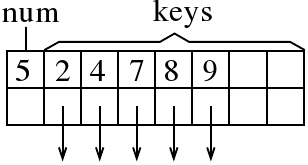
\includegraphics[scale=0.25]{images/ordered.png} \\
Unordered & \\
& 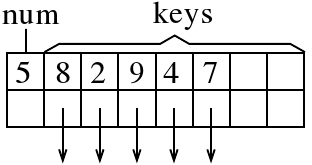
\includegraphics[scale=0.25]{images/unordered.png} \\
Bitmap & \\
&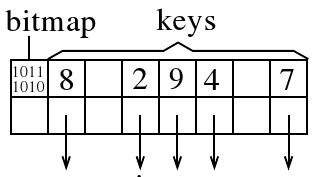
\includegraphics[scale=0.25]{images/bitmap.png}
\end{tabular}


\end{frame}



\subsection{$B^+$-Tree Variants}
\begin{frame}
\frametitle{Variants}

\begin{itemize}
\item Sorted
\item Unsorted
\item Unsorted Leaf
\item Unsored Leaf with bitmap
\end{itemize}

\end{frame}
\section{Hash Join}

\begin{frame}
\frametitle{SS}

\begin{itemize}
\item .
\end{itemize}

\end{frame}

\subsection{Simple Hash Join}
\begin{frame}
\frametitle{SS}

\begin{itemize}
\item .
\end{itemize}

\end{frame}


\subsection{Cache Partitioning}

\begin{frame}
\frametitle{SS}

\begin{itemize}
\item .
\end{itemize}

\end{frame}



\subsection{Virtual Cache Partitioning}

\begin{frame}
\frametitle{SS}

\begin{itemize}
\item .
\end{itemize}

\end{frame}
\section{Experimental Results}

\begin{frame}
\frametitle{Setting} %Intro/purpose of this section}

\begin{itemize}
\item .
\end{itemize}

\end{frame}

\subsection{$B^+$-Tree}

\begin{frame}
\frametitle{SS}

\begin{itemize}
\item .
\end{itemize}

\end{frame}
\subsection{Hash Join}

\begin{frame}
\frametitle{SS}

\begin{itemize}
\item .
\end{itemize}

\end{frame}



\subsection{Conclusion}

\begin{frame}
\frametitle{SS}

\begin{itemize}
\item .
\end{itemize}

\end{frame}
\end{document}

%General
%
%    * Is it clear where the paper was published and by whom?
%    * Does the talk have a concrete motivating example very early?
%    * Are unfamiliar abbreviations introduced and used appropriately?
%    * Is the main problem addressed in the paper clearly stated?
%    * Does the presentation have concrete and minimal examples of core ideas?
%    * Are dynamics, e.g., searching a tree presented using animation techniques?
%    * Are the listeners background use appropriately, e.g., no need to tell what an array is, however must tell what the XY++-Tree is?
%    * Is there a reasonable number of slides in total in the presentation?
%
%Figures
%
%    * Are complicated figures presented in sufficient details?
%    * Are the symbols used in the figures clear to the listeners?
%
%Performance Graphs
%
%    * Is data, queries, modification, and transactions appropriately introduced?
%    * Are the axis on performance graphs clearly explained?
%    * Are the main conclusion from the graph clearly stated?
%    * Is there only one graph per slide (or are graphs compared)?
%
%Critique
%
%    * Is the critique relevant and fair?
%    * Is the critique balanced?
%    * Is the critique points concrete, i.e., not "it is a good paper"?
